% !TeX root = ../main.tex

\chapter{Real-Time Recurrent Learning}

À partir de cette section, on va chercher à reconnaître une chaîne de caractère en temps réel : c'est à dire que en donnant un ou plusieurs caractères, on doit être capable de prédire la fin de la chaine, ou tout du moins un fin possible, selon une grammaire prédéfinie.
Pour résoudre ce genre de problème, on utilise des réseaux neuronaux récurrents, qui vont permettre de se souvenir des états précédents pour pouvoir prédire efficacement les états suivants ; on ajoute donc une notion de mémoire au réseau.
Dans un premier temps, nous allons nous intéresser aux réseaux récurrents simples, et à deux algorithmes qui vont permettre d'ajuster les poids du réseau: Real-Time Recurrent Learning (RTRL) et BackPropagation Through Time (BPTT).

\section{Théorie}

Dans la suite, nous allons nous intéresser à la grammaire de Reber, qui nous fournira des échantillons de test pour la suite.

\subsection{La grammaire de Reber}

Une grammaire de Reber est un langage défini par l'automate déterministe cyclique suivant :

\begin{figure}[!ht]
\begin{center}
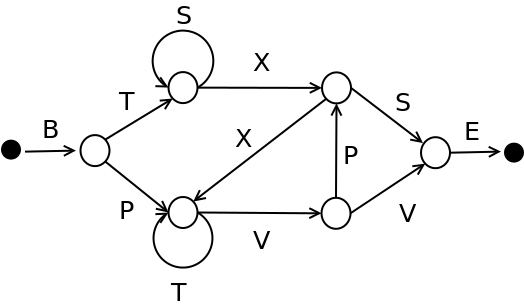
\includegraphics[width=0.6\textwidth]{images/reberGrammar.png}
\end{center}
\caption{Grammaire de Reber simple}
% TODO : Include credits
\end{figure}


On considère une probabilité uniforme de choisir l'état suivant parmi les états suivants possibles.
La lettre $B$ et la lettre $E$ sont des lettres indiquant simplement le début et la fin de la chaîne, elles n'ont pas d'intérêt propre pour la grammaire.
Les autres lettres présentes sur les arêtes peuvent varier, mais elles doivent respecter les règles suivantes :

\medskip

\begin{itemize}
	\item Chaque lettre doit apparaitre exactement deux fois ;
	\item On ne peut pas obtenir deux lettres consécutives en passant par des états différents.
\end{itemize}

\medskip

L'intérêt de la grammaire de Reber est qu'il s'agit un automate simple qui ne nécessite que la mémoire de la dernière et de l'avant dernière lettre pour déterminer les lettres suivantes possibles.
En effet, d'après la dernière règle, connaitre les deux dernières lettres impose l'état actuel dans l'automate.
En outre, chaque lettre apparaissant deux fois, la connaissance seule de la dernière lettre ne suffit pas à prédire la suivante correctement.
On remarque que l'on peut résoudre ce problème avec un perceptron classique si on donne en entrée du perceptron les deux dernières lettres du mot. Cependant cette approche reste un bricolage propre à ce cas, et n'est pas du tout généralisable. On va donc chercher ici à résoudre ce problème en passant en entrée du réseau chaque lettre l'une après l'autre, à l'aide de la mémoire du réseau. Nous pourront ensuite utiliser des modèles de grammaire plus complexes, comme la grammaire de Reber symmétrique.

\medskip

Le problème de la grammaire symmétrique est un problème similaire à la grammaire simple. L'automate le représentant est :

\begin{figure}[!ht]
\begin{center}
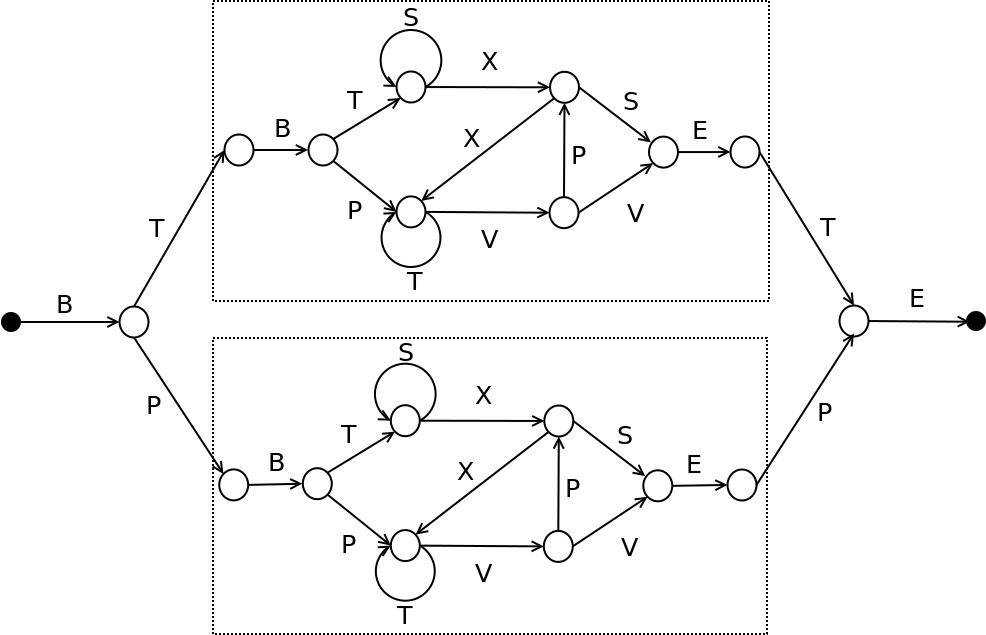
\includegraphics[width=0.6\textwidth]{images/reberGrammarSymmetric.png}
\end{center}
\caption{Grammaire de Reber symétrique}
\end{figure}

On remarque qu'il est constitué de deux grammaires de Reber simples qui sont reliées uniquement en entrée et en sortie.
La difficulté de ce problème est qu'il faut mémoriser, et se rappeler de la première valeur pour déterminer la dernière.
Dans ce cas, une mémoire infinie, au tout du moins dépassant le court terme, est nécessaire pour se souvenir de la première entrée.
Il est ici impensable d'utiliser de la même façon un réseau de perceptron classique. On a alors besoin d'un réseau récurrent, dont la sortie à un instant $t$ va dépendre de la sortie à un instant $t-1$.

\subsection{Réseaux neuronal récurrents}

Le principe d'un réseau neuronal récurrent est d'utiliser le résultat obtenue par la sortie précédente à l'entrée du calcul suivant.
On aura donc en appelant $x(t)$ la donnée en entrée à l'instant $t$ et $y(t)$ la sortie associé.
On a alors $y(t) = f(x(t), y(t-1))$.
En appelant $\alpha$ un paramètre de la fonction $f$.
Le but est de faire un apprentissage sur $\alpha$ pour minimiser à chaque temps $t$ l'erreur $E(t)$ entre la sortie théorique et la sortie pratique.
De la même façon que précédemment, on va donc calculer $\cfrac{\partial E(t)}{\partial \alpha}$ pour utiliser la méthode du gradient :
Nous allons nous intéresser au cas où $f$ est de la forme :

\[ f(x(t), y(t-1)) = \sigma\left (W x(t) + R y(t-1) + b\right )\]

Avec $W$, $R$ qui sont des matrices de poids, $b$ un biais et $\sigma$ une fonction d'activation.
On reconnait donc d'après ce qui précède la formule d'un réseau perceptron à $0$ couche caché et "fully connected".
On pose $\overline{y(t)} = W\times x(t) + R\times y(t-1) + b$.
Les paramètres du systèmes sont donc les éléments de la matrice
On obtient donc pour l'apprentissage :

\[\cfrac{\partial E(t)}{\partial \alpha} = \left\langle \cfrac{\partial y(t)}{\partial \alpha}, J_E \right\rangle\]

\begin{figure}[!ht]
\begin{center}
  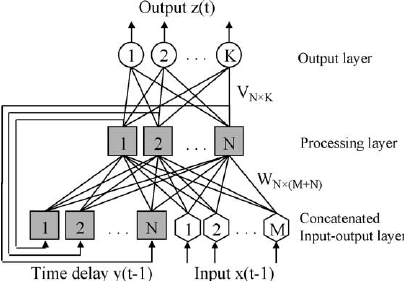
\includegraphics[width=0.5\textwidth]{images/rtrl.png}
\end{center}
\caption{Réseau récurrent RTRL}
\end{figure}

Cependant ici, à cause de la nature bouclée du réseau, l'algorithme de rétro-propagation simple vu ci-dessus ne peut s'appliquer. Nous allons donc commencer par étudier l'algorithme Real-Time Reculent Learning, ou RTRL, qui permet de calculer les erreurs en temps réel.

\section{Algorithme RTRL}
Le premier algorithme est aussi le plus simple mathématiquement, mais comme on va le voir cela va de pair avec une complexité temporelle et spatiale élevée.

Afin de prendre en compte les biais simplement, on considerera une entrée supplémentaire de valeur toujours égale à $1$, et connectée à tous les neurones du réseau. Ainsi, le vecteur des biais $b$ sera les poids correspondant à cette entrée unitaire.

On suppose donc que l'on dispose de $m$ entrées (dont une unitaire pour les biais), prenant les valeurs $\boldsymbol{x}(t)$ à l'instant $t$. Ces entrées sont reliées à $n$ neurones, dont les sorties sont notées $\boldsymbol{y}(t)$ à l'instant $t$. Par commodité, on note $\boldsymbol{z}(t)$ la concaténation de $\boldsymbol{x}(t)$ et de $\boldsymbol{y}(t)$. Soit de plus les ensembles $I$ l'ensemble des entrées et $U$ l'ensemble des neurones, tels que

\[ z_k(t) = \begin{cases}
                  x_k(t) & \text{si }k \in I\\
                  y_k(t) & \text{si }k \in U\\
                \end{cases}
\]

Ainsi, on peut définir une unique matrice de poids $\boldsymbol{W}=(w_{i,j})$, de taille $n\times(m+n)$. On considérera que le temps $t$ est discret.

On pose ensuite
\[ s_k(t) = \sum_{i \in I \cup U} w_{k,i}z_i(t) \]
le vecteur des entrées pondérées à l'instant $t$, et on obtient par construction
\[ y_k(t+1) = f_k(s_k(t)) \hspace*{1cm} \forall k \in U \]
le vecteur des sorties à l'instant $t+1$. La fonction $f_k$, pour tout $k \in U$, est la fonction d'activation du neurone $k$. Nous prendrons ici la fonction sigmoïde comme fonction d'activation: pour tout $k \in U$ et $t > 0$, $f_k(t) = \frac{1}{1+e^{-t}}$.

Nous avons maintenant défini l'évolution du réseau en fonction du temps grâce aux équation ci-dessus. On va maintenant chercher à estimer, puis propager l'erreur dans le réseau.

Soit $T(t)$ l'ensemble dont on connaît \textit{a priori} la valeur à l'instant $t$ ; il s'agit simplement des neurones de sortie dont la valeur est imposée par l'apprentissage. On remarque que cet ensemble des neurones de sortie peut varier au cours du temps, bien que cela ne soit pas nécessaire dans le cadre de l'apprentissage des grammaires de Reber. On note de plus, pour tout $k in T(t)$, la valeur attendue $d_k(t)$ en sortie du neurone $k$ à l'instant $t$.

On définit alors l'erreur $e_k(t)$, pour tout neurone $k$, par :
\[ e_k(t) =  \begin{cases}
                  d_k(t) - y_k(t) & \text{si }k \in T(t)\\
                  0 & \text{sinon}\\
                \end{cases}
\]

En prenant pour fonction de coût l'erreur quadratique moyenne, la quantité à minimiser au court du temps s'écrit
\[ J(t) = \tfrac{1}{2} \sum_{k \in U} e_k^2(t) \]
et l'objectif est de minimiser la quantité totale
\[ J_{\text{total}} = \sum_{t} J(t) \]

On procède pour cela par une descente de gradient sur les poids $\boldsymbol{W}$, en les ajustant de temps en temps d'une valeur $\Delta w_{i,j}$.

Pour cela, on s'intéresse à la variation de l'erreur due au poids $w_{i,j}$ à l'instant $t$, à un facteur d'apprentissage $\alpha > 0$ près :
\[ \Delta w_{i,j}(t) = -\alpha \frac{\partial J(t)}{\partial w_{i,j}} \]
Et bien sûr, $\Delta w_{i,j} = \sum_t \Delta w_{i,j}(t)$.

Or on a
\[ -\frac{\partial J(t)}{\partial w_{i,j}} = \sum_k \left( e_k(t) \times \frac{\partial y_k(t)}{\partial w_{i,j}} \right) \]
et à l'aide des équations qui régissent la propagation il vient que, pour tout $k \in U$, $i \in U$ et $j \in I \cup U$,
\[ \frac{\partial y_k(t+1)}{\partial w_{i,j}} = f'_k(s_k(t)) \times \sum_{l \in U} \left( w_{k,l} \frac{\partial y_l(t)}{\partial w_{i,j}} + \delta_{i,k} z_j(t) \right) \]
où $\delta_{i,k}$ est la fonction delta de Kronecker (égale à $1$ si $i = k$, et nulle sinon), et, si $f$ est la fonction sigmoïde, $f'_k(s_k(t)) = y_k(t) \times (1 - y_k(t))$.

Cette équation récurrente en $\left( \frac{\partial y_l(t)}{\partial w_{i,j}} \right)_t$ va nous permettre de tout calculer par la suite, puisque l'on sait de plus qu'en $t=0$, cette quantité $\frac{\partial y_l(0)}{\partial w_{i,j}}$ est nulle.

En posant
\[ p_{i,j}^k(t) = \frac{\partial y_l(t)}{\partial w_{i,j}} \hspace*{1cm} \text{ et }p_{i,j}^k(0) = 0 \]
l'équation ci-dessus se réécrit
\[ p_{i,j}^k(t+1) = f'_k(s_k(t)) \times \sum_{l \in U} \left( w_{k,l} p_{i,j}^l(t) + \delta_{i,k} z_j(t) \right) \]
et dans le cas de la fonction sigmoïde
\[ p_{i,j}^k(t+1) = y_k(t) (1 - y_k(t)) \times \sum_{l \in U} \left( w_{k,l} p_{i,j}^l(t) + \delta_{i,k} z_j(t) \right) \]
Enfin, les variations de poids se notent alors
\[ \Delta w_{i,j}(t) = -\alpha \sum_{k \in U} e_k(t) p_{i,j}^k(t) \]

On voit donc que l'on arrive à calculer $\Delta w_{i,j}$ itérativement pour chaque pas de temps $t$. L'implémentation de l'algorithme va donc consister à calculer itérativement toutes les valeurs utiles afin de déterminer les $p_{i,j}^k(t)$.

La complexité de cet algorithme est en $O(n^3(n+m))$, à le calcul de $p_{i,j}^k(t)$ se faisant pour tout $i$, $j$, $k$ et demandant une somme de $n$ éléments. En espace, la complexité est de $O(n^2(n+m))$.

\section{Implémentation}
\subsection{Structure du code}

Une première tentative d'implémentation a consisté à adapter le code du programme précédent, utilisé pour les réseaux neuronaux simples, aux réseaux neuronaux récurrents. Cependant, après de longues semaines de déboggage sans résultats probants, nous avons décider de commencer un nouveau programme le plus simple possible, intitulé \textit{SimpleRTRL}.

À cette fin, nous avons utilisé la bibliothèque C++ Eigen, qui contient toutes les structures et algorithmes nécessaires à l'algèbre linéaire. Le diagramme de classes UML est présenté ci-dessous:

\begin{figure}[!ht]
\begin{center}
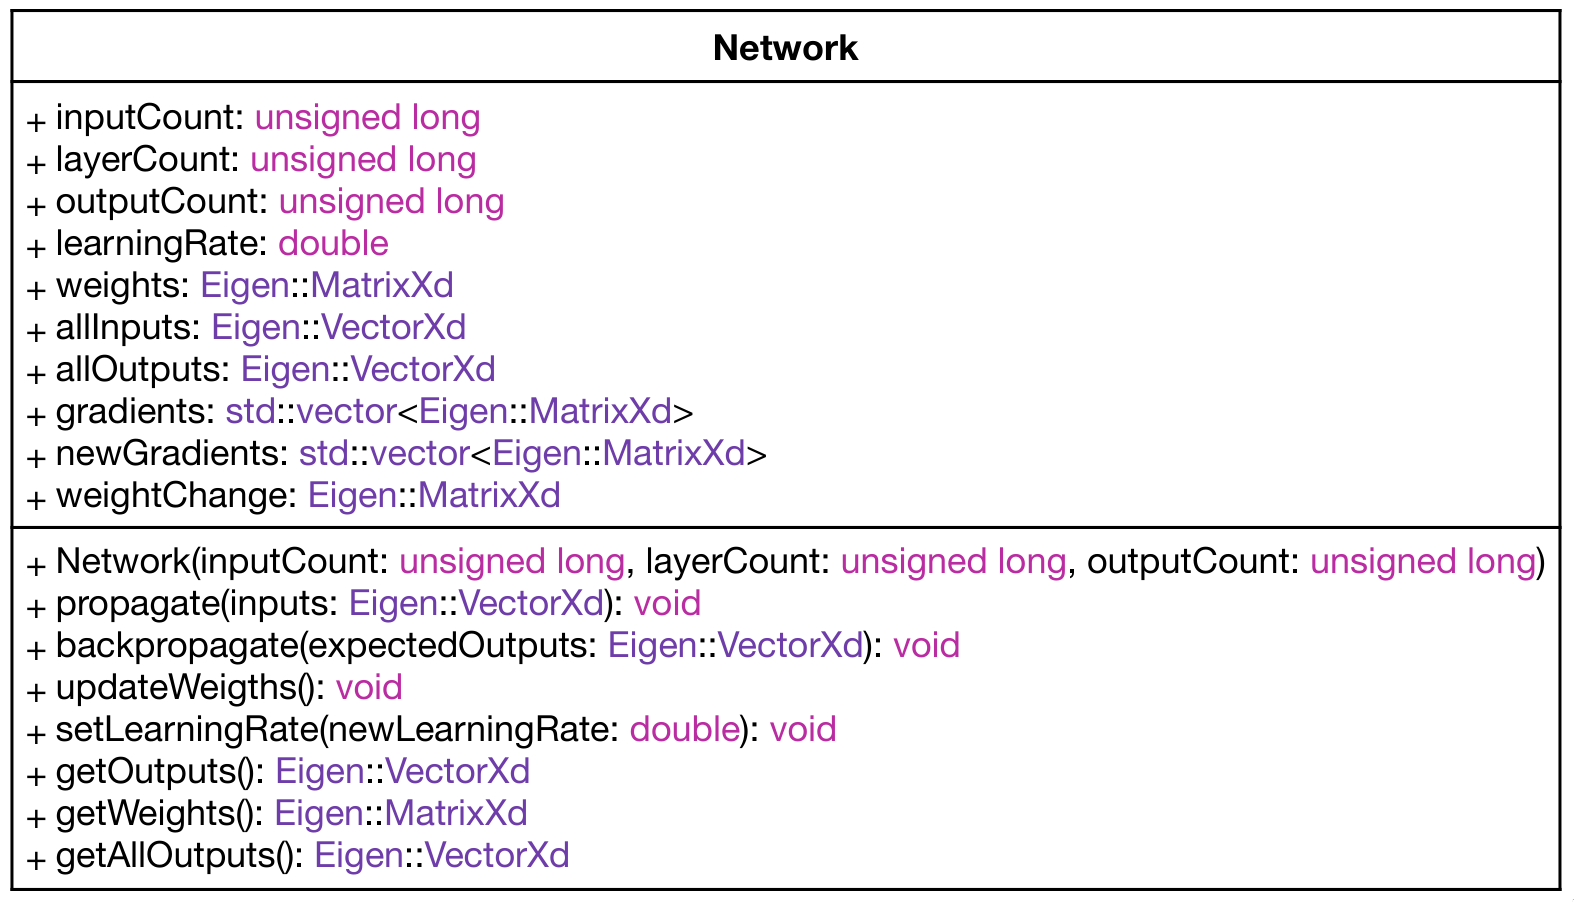
\includegraphics[width=0.6\textwidth]{images/SimpleRTRL-UML.png}
\end{center}
\caption{Diagramme de classes de \textit{SimpleRTRL}}
\end{figure}

On voit donc qu'il y a une unique classe, \verb+network+, qui effectuera tous les calculs, selon les étapes suivantes:
\begin{itemize}
	\item on initialise un réseau avec \verb+inputCount+ entrées et \verb+layerCount+ neurones dont \verb+outputCount+ seront considérés comme des sorties
	\item on propage un vecteur d'entrées \verb+inputs+ dans le réseau avec la méthode \verb+propagate+
	\item on rétro-propage l'erreur avec la méthode \verb+backpropagate+ à l'aide du vecteur des sorties attendues \verb+expectedOutputs+
	\item après avoir propagé et rétro-proagé plusieurs fois, on applique les changements de poids avec \verb+updateWeights+
\end{itemize}
À tout moment, on peut récupérer les sorties avec \verb+getOuputs+, ou plus générallement voir l'état du réseau avec les accesseurs. Lorsque les changements de poids sont effectués, toutes les données intermédiaires sont effacées et on revient à l'instant initial $t=0$.

Les poids du réseau sont initialisés avec une valeur entre $-0.1$ et $0.1$. L'ensemble des sorties des neurones sont stockés dans une unique liste, dont les $n'=|T(t)|$ premiers sont considérés comme des neurones de sortie.

\subsection{Structure du réseau utilsée}
Afin de faire de réaliser l'apprentissage, on utilise une liste de 2,4 millions de mots générés à partir de la grammaire de Reber simple et autant générés à partir de la grammaire double. Pour les tests, on utilise une liste disctincte de 1 million de mots pour chaque grammaire.

Afin de tester l'apprentissage des grammaires de Reber par les réseaux récurrents et l'algorithme RTRL, nous avons choisi une certaine structure de réseau. Celle ci consiste à mettre une entrée par lettre possible (en l'occurence, 7 : \verb+B+, \verb+T+, \verb+P+, \verb+S+, \verb+X+, \verb+V+ et \verb+E+), et autant de sorties, avec au total 30 neurones (dont 7 considérés comme des neurones de sortie). Ensuite, à chaque instant, l'entrée correspondant à la lettre courante est mise à $1$, et les autres à $0$. La propagation est réalisée, puis la rétro-propagation, et enfin, lorsqu'on a fait passer le mot entier de cette façon, on applique les variations de poids, avec un facteur d'apprentissage de $0.1$.

Pour valider cet apprentissage, on procède de même mais sans rétro-propagation ni apprentissage. Les lettres indiquées en sortie par le réseau sont celles dont les sorties correspondantes ont une valeur supérieur à un seuil, fixé à $0.3$.

Des fonctions utilitaires permettent de réaliser l'apprentissage puis de le tester dans le cadre des grammaires de Reber. Elles enchaînent l'apprentissage de 50 mots différents par un test du réseau sur 1000 mots, le tout répété 2000 fois. Pour chaque test, on vérifie que la lettre suivante du mot est bien parmi les lettres suivantes possibles selon le réseau (c'est-à-dire une sortie dont la valeur est supérieure au seuil de $0.3$). Le score final de réussite est le nombre de lettres prédites correctement sur le nombre total de lettres, et on suit l'évolution de ce score au fur et à mesure des apprentissages.

Dans le cas des grammaires doubles, on fait de même en se restreignant uniquement à vérifier la prédiction de l'avant-dernière lettre, celle que l'on ne peut trouver qu'en se souvenant de la seconde lettre du mot.

\subsection{Exemple}
Voici un exemple pour illustrer le processus ci-dessus. Supposons que l'on veuille apprendre le mot \verb+BPVPSE+.

On propage donc le vecteur d'entrée $(1, 0, 0, 0, 0, 0, 0)$ (qui correspond à $1$ pour l'entrée de la lettre \verb+B+ et $0$ pour les autres). En sortie, on obtient le vecteur $\boldsymbol{y}(0)$, que l'on fixe ici par exemple à $\boldsymbol{y}(0)=(0.1, 0.2, 0.5, 0.2, 0.6, 0.1, 0.1)$ (ce qui correspond à $0.1$ pour \verb+B+, $0.2$ pour \verb+T+, $0.5$ pour \verb+P+, $0.2$ pour \verb+S+, $0.6$ pour \verb+X+, $0.1$ pour \verb+V+ et $0.1$ pour \verb+E+). Dans ce cas, le réseau à bien prédit la lettre \verb+P+ comme étant possible (car $0.5>0.3$), mais il n'a pas prédit correctement l'autre possibilité : il estime que \verb+T+ n'est pas possible (alors que c'est le cas), mais que \verb+X+ est possible (ce qui n'est pas le cas).

Pour la rétro-propagation, on lui donne le vecteur des sorties désirées $\boldsymbol{d}(0)=(0, 0, 1, 0, 0, 0, 0)$, puisque la lettre suivante est un \verb+P+. Le réseau pourra apprendre que \verb+T+ est une autre lettre possible après un \verb+B+ initial avec d'autre mots. Une fois la rétro-propagation réalisée, on met en entrée $y(1)=d(0)$, et ainsi de suite.

Une fois que l'on a propagé et rétro-propagé chaque lettre du mot, on effectue les changements de poids avec les variations calculées pour chaque lettre.

Lors des tests, si la lettre suivante est effectivement prédite, comme c'est le cas ci-dessus, on comptabilise un point. En revanche, si on avait une sortie de $0.1$ associée à la lettre \verb+P+, le point ne serait pas comptabilisé.

\section{Résultats}
Étudions maintenant les résultats obtenus pour l'apprentissage des grammaires de Reber simples et doubles.

\subsection{Grammaire de Reber simple}
On réalise 100 apprentissages successifs et indépendants de 100000 mots chacun, en testant l'apprentissage tout les 50 mots, dans les conditions décrites ci-dessus. On obtient la courbe du taux de prédiction de lettre suivante ci-dessous, avec en bleu la moyenne sur les 100 essais et en gris le taux de confiance à 95\%. L'échelle des ordonnées est en pourcentages.

\begin{figure}[!ht]
\begin{center}
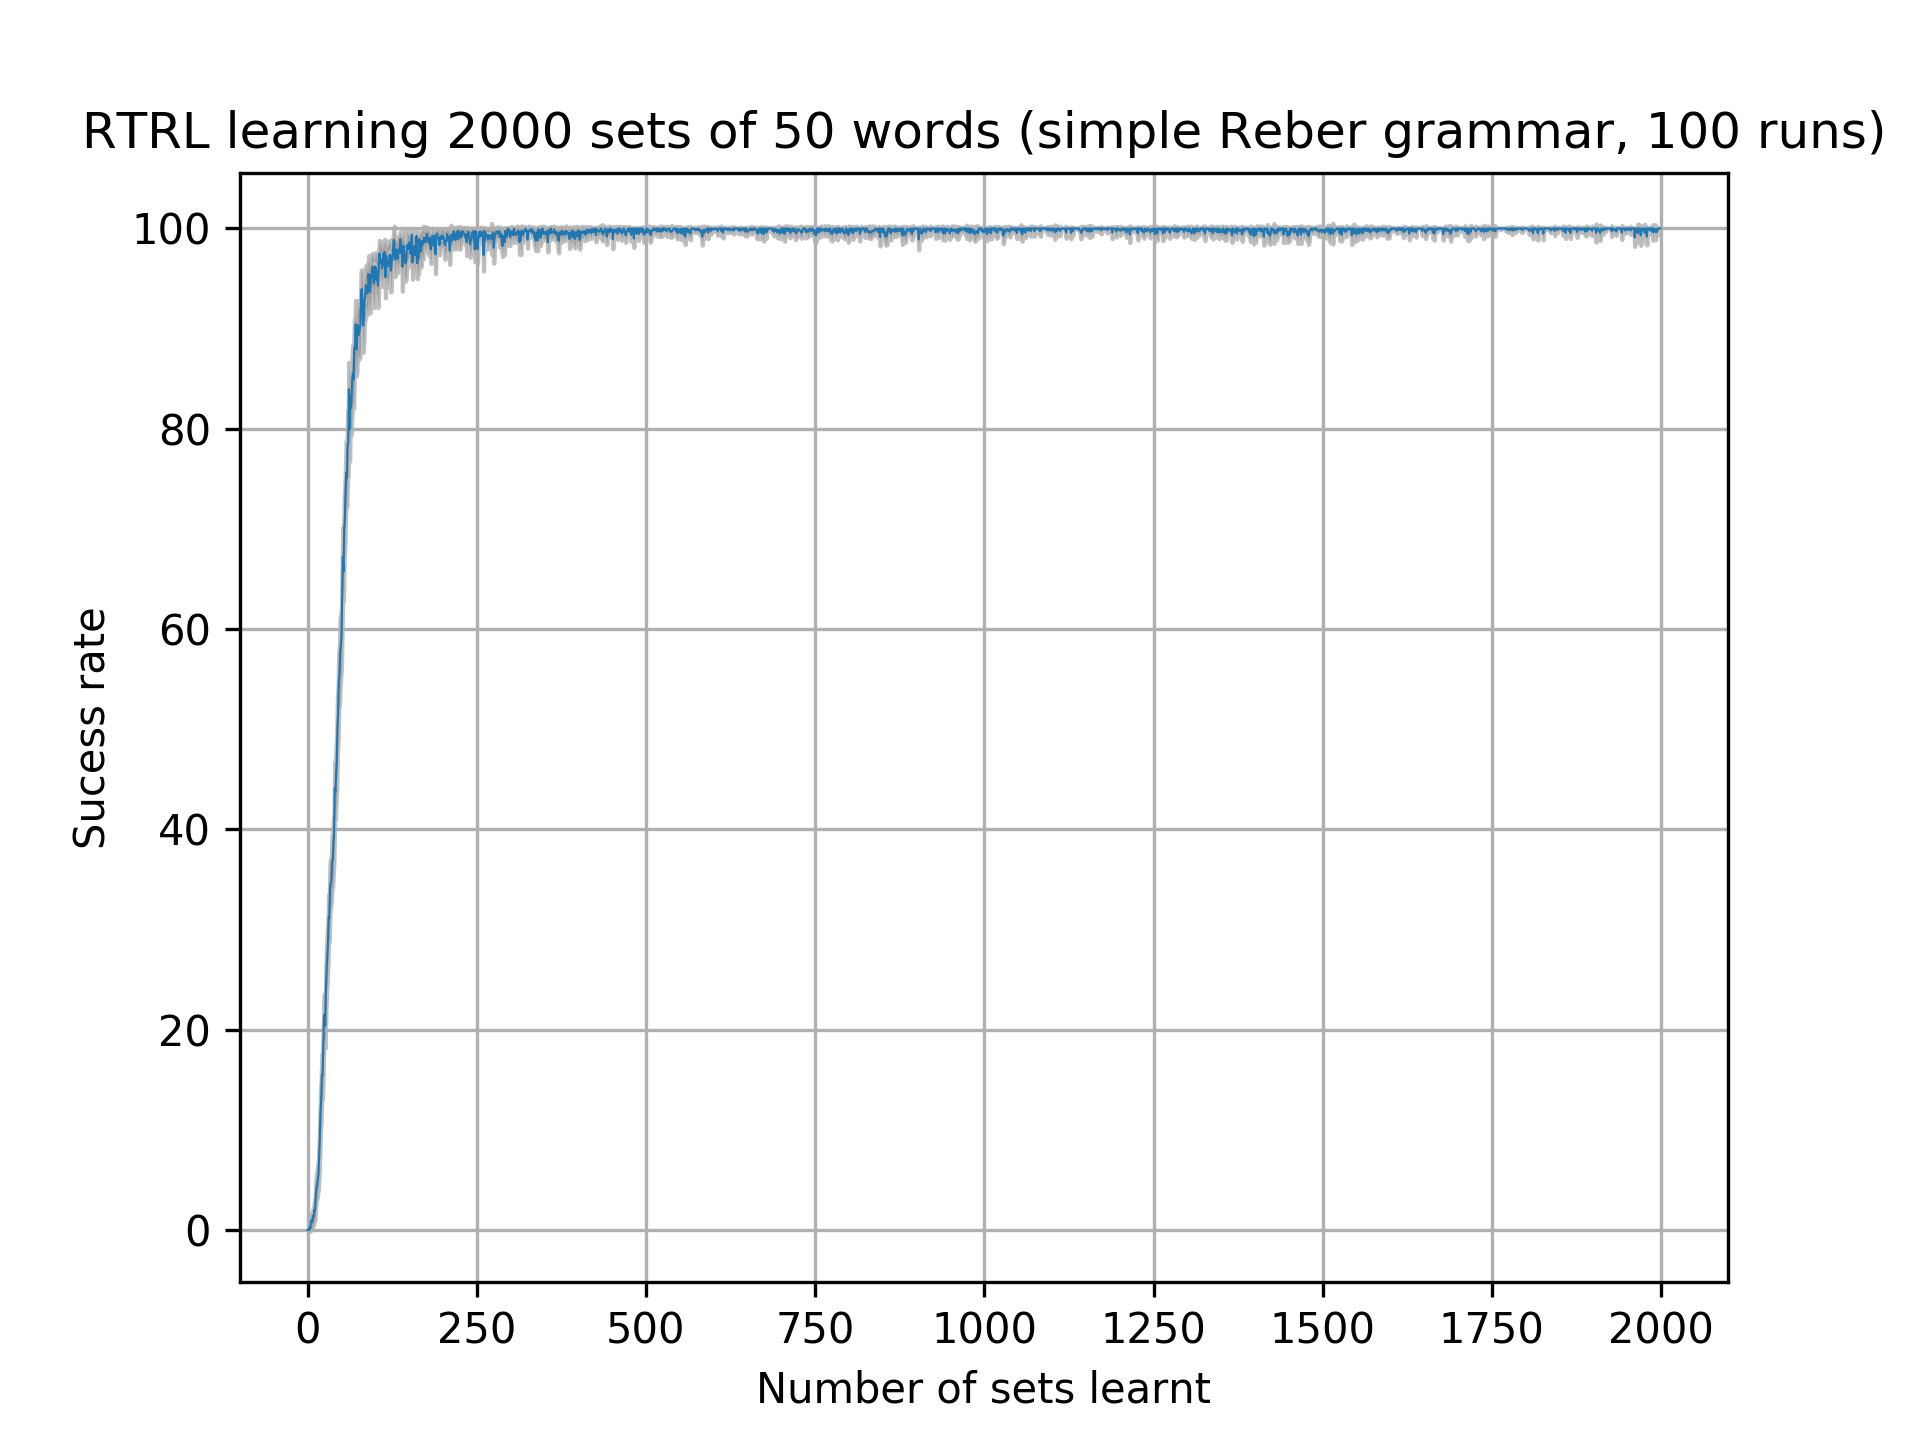
\includegraphics[width=0.6\textwidth]{images/SimpleRTRL-r1.png}
\end{center}
\caption{Taux de succès au cours de l'apprentissage de la grammaire simple}
\end{figure}

On remarque que l'apprentissage est de bonne qualité, et que le réseau arrive sans problème deviner la suite du mots dès le 500\textsuperscript{ème} test, c'est-à-dire après avoir appris 25000 mots.

La durée d'un essai complet est d'environ 30 minutes sur un cœur Intel® Xeon® cadencé à $2.40$ GHz.

\subsection{Grammaire de Reber double}
De même que pour la grammaire simple, on réalise 100 apprentissages successifs et indépendants de 100000 mots, en testant l'apprentissage tout les 50 mots. On obtient la courbe du taux de prédiction de l'avant-dernière lettre en figure 3.6, avec en bleu la moyenne sur les 100 essais et en gris le taux de confiance à 95\%. L'échelle des ordonnées est en pourcentages.

\begin{figure}[!ht]
\begin{center}
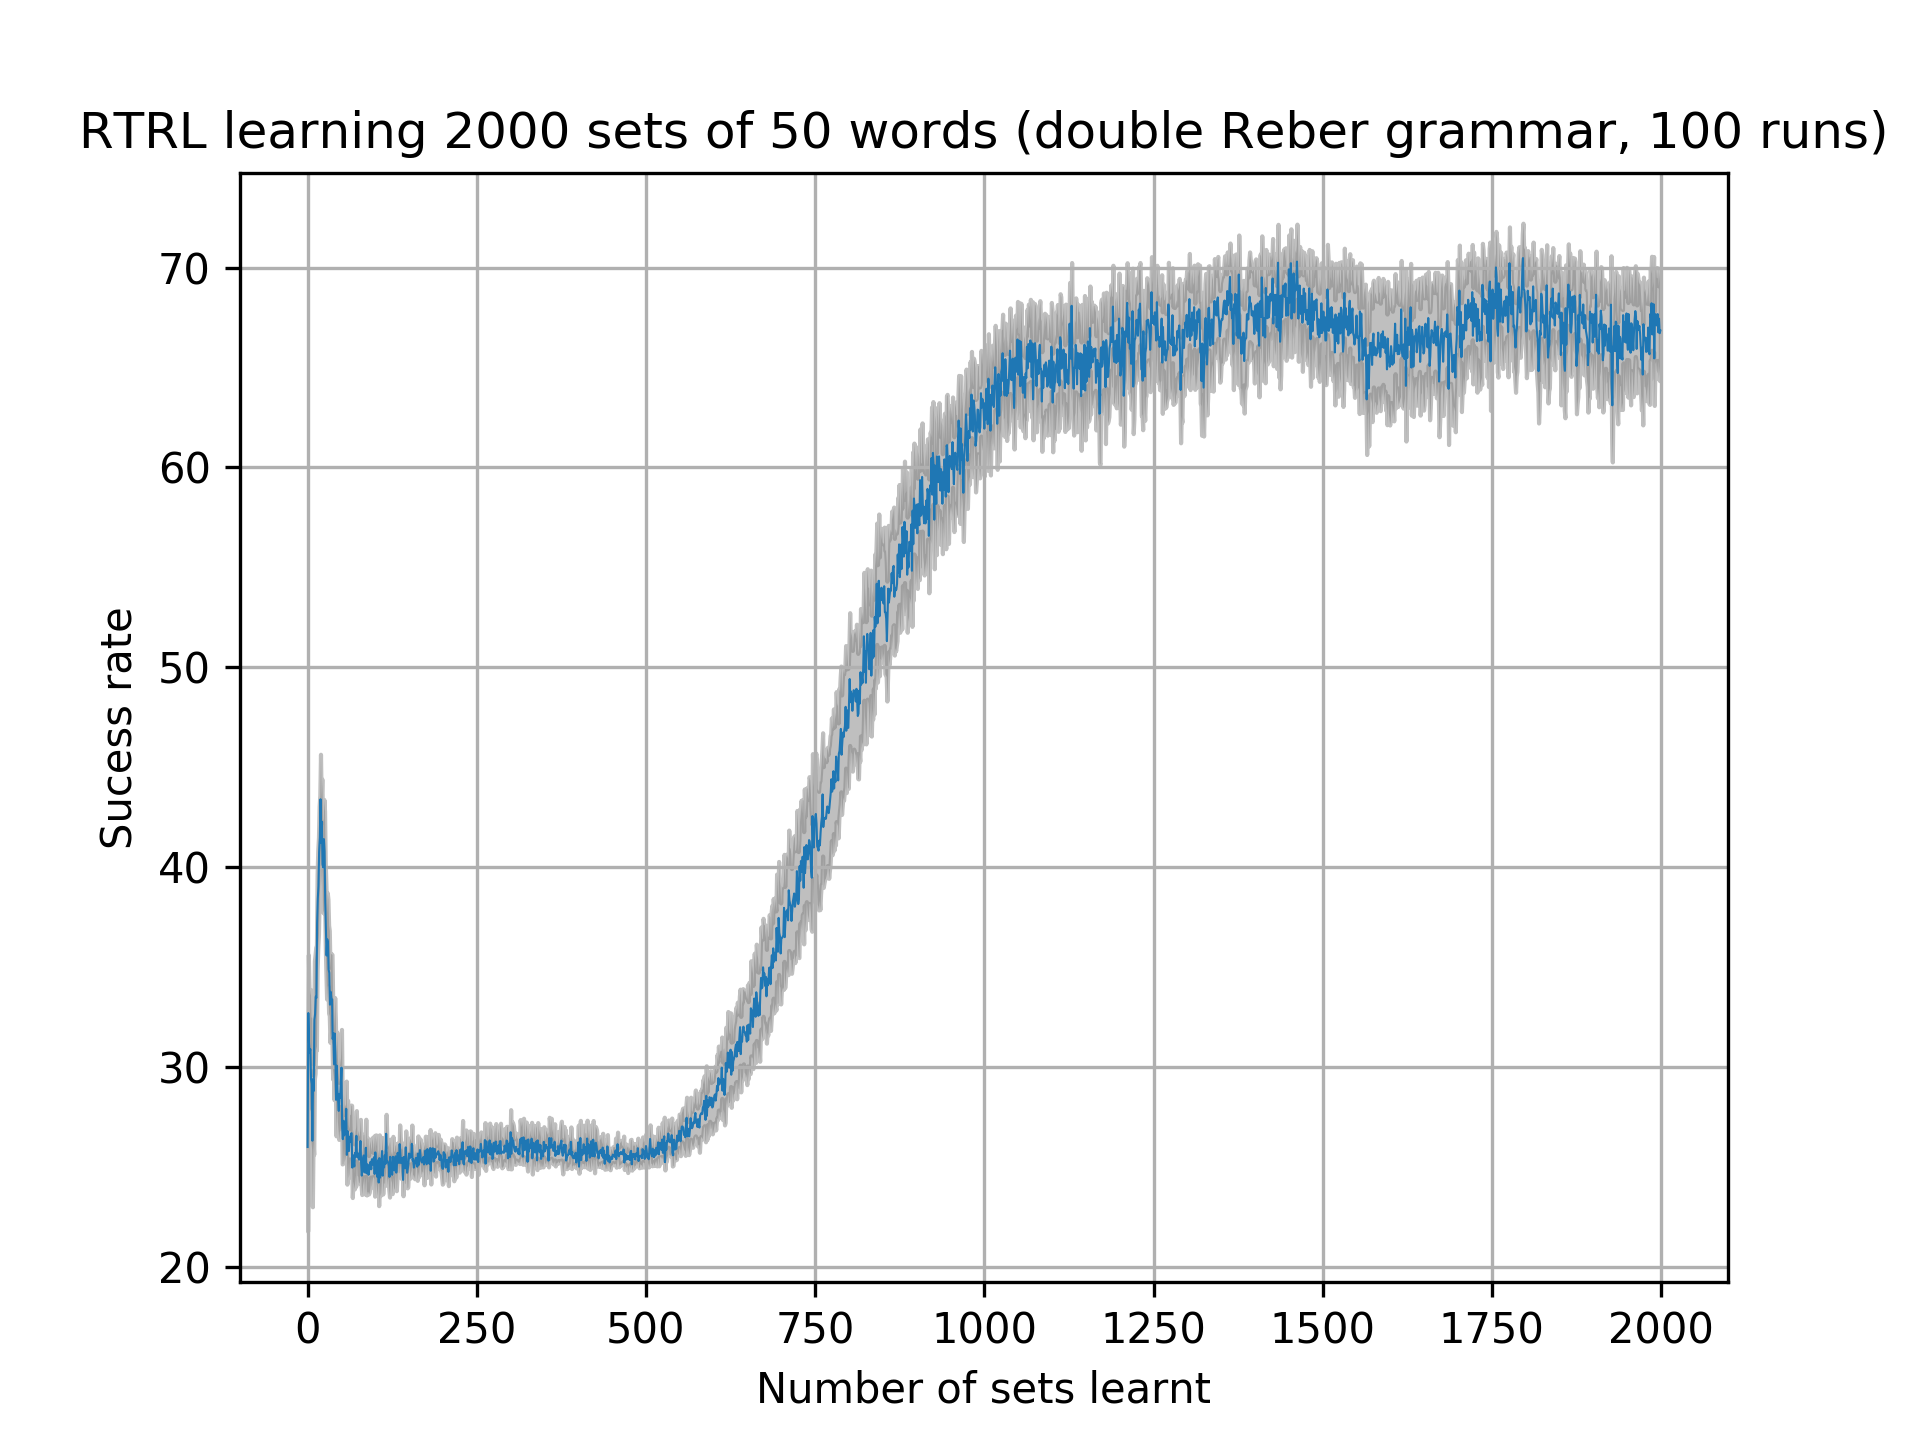
\includegraphics[width=0.6\textwidth]{images/SimpleRTRL-r2.png}
\end{center}
\caption{Taux de succès au cours de l'apprentissage de la grammaire double}
\end{figure}

La durée d'un essai complet est d'environ 40 minutes sur un cœur Intel® Xeon® cadencé à $2.40$ GHz.

Ici, l'apprentissage est de moindre qualité, on voit immédiatement que le réseau a plus de difficultés pour apprendre cette grammaire, et qu'il n'y arrive asymptotiquement pas. Il y a tout d'abord un plateau jusqu'au 750\textsuperscript{ème} test environ, où le taux de succès stagne autour de 25\%, puis il augmente progressivement jusqu'à atteindre 70\%. Là, la marge de confiance à 95\% reste élevée ; en effet de nombreux essais présentent des comportements erratiques où le taux de réussite redescend subitement vers 25\%, avant de remonter. La figure 3.7 présente un tel essai.

\begin{figure}[!ht]
\begin{center}
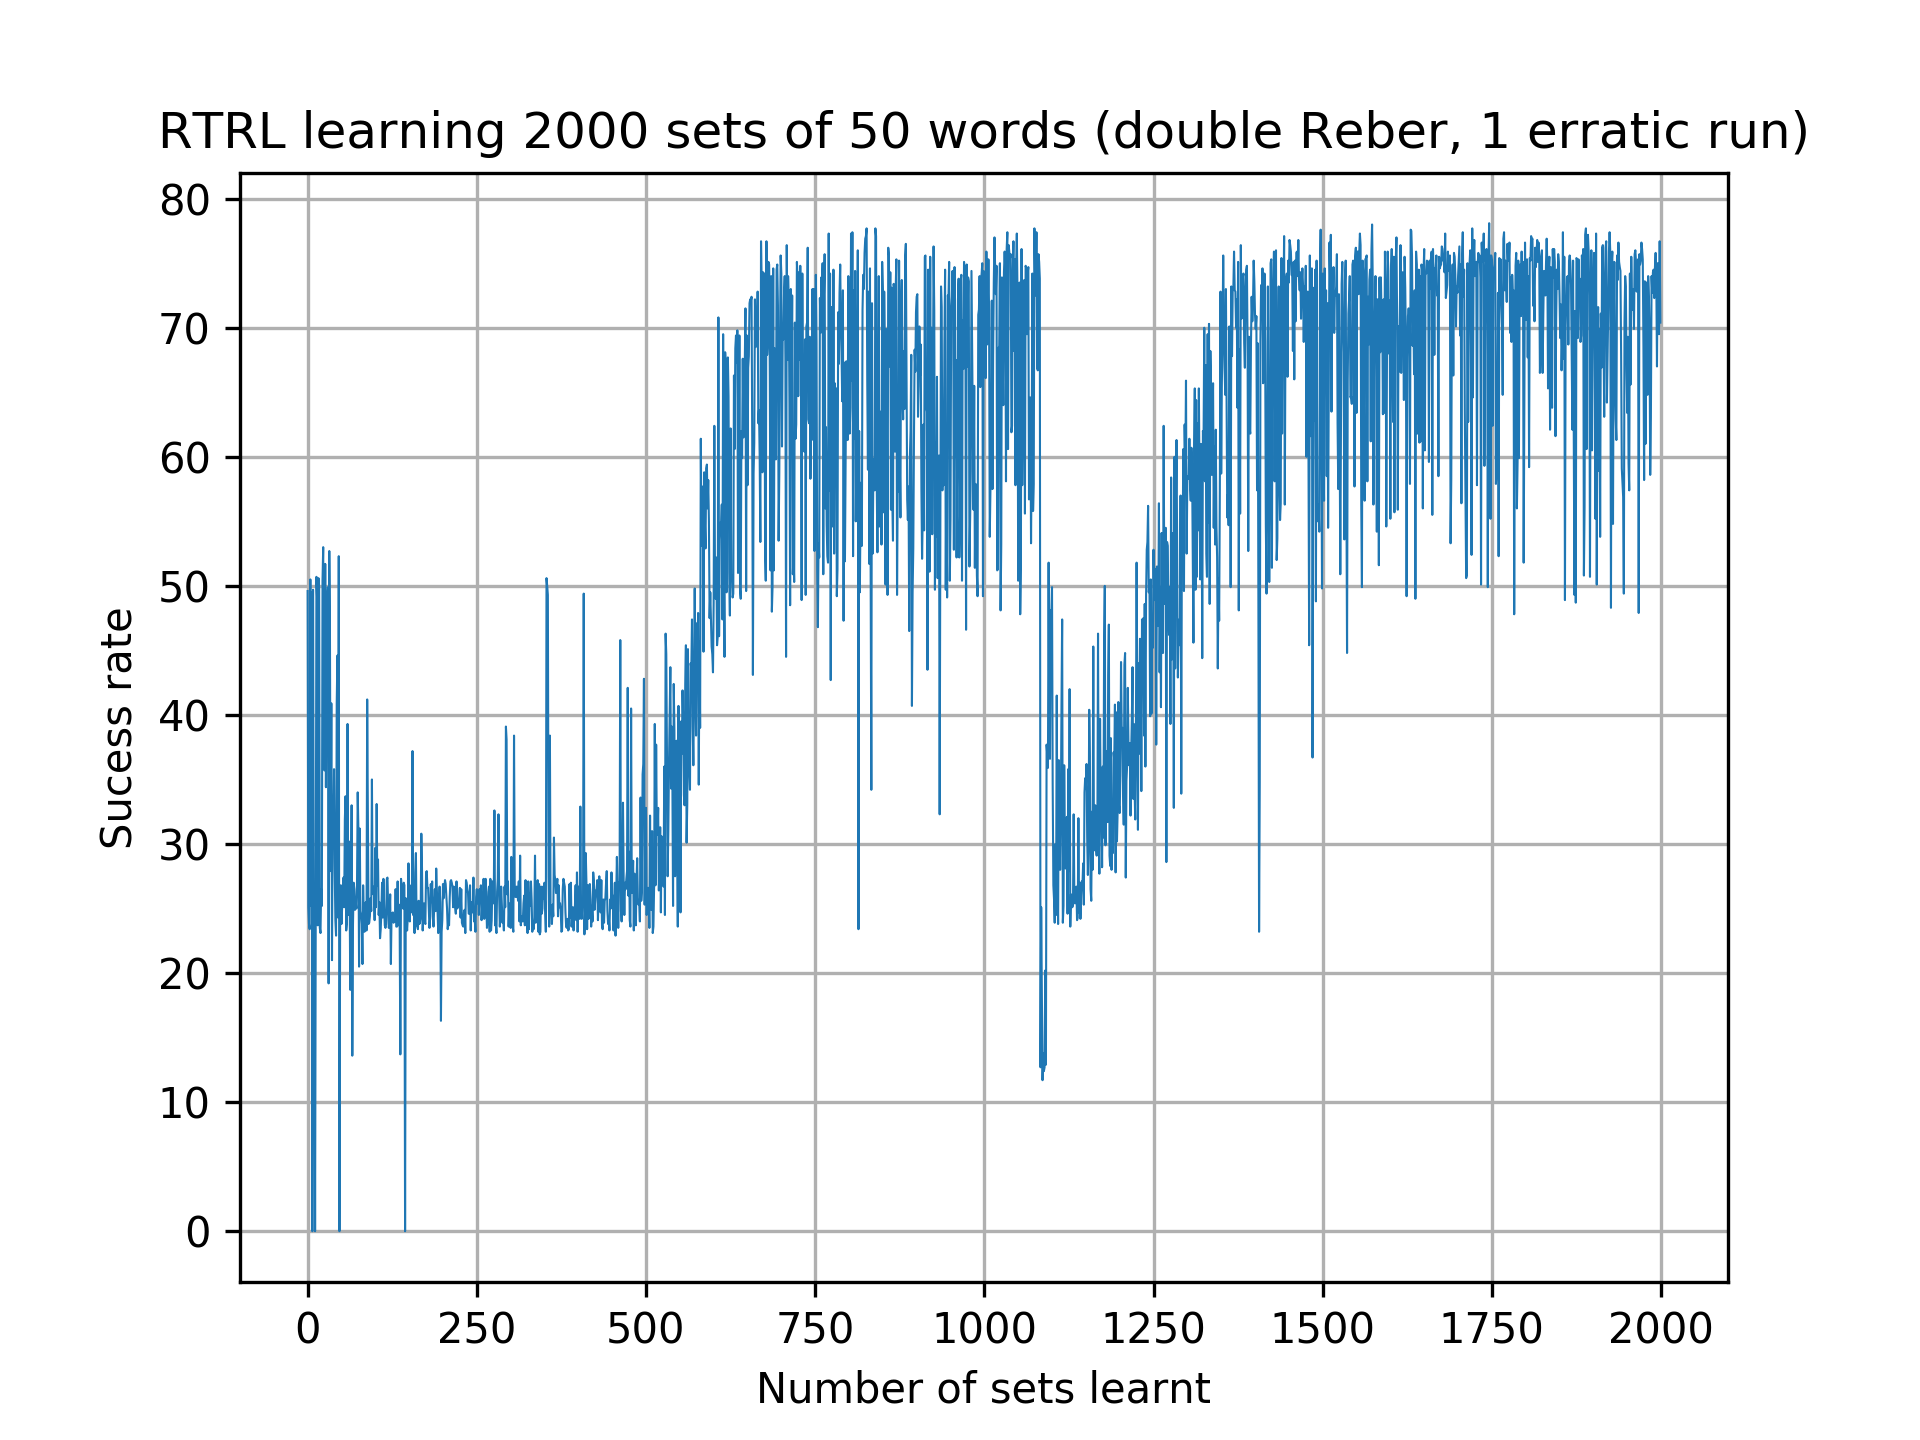
\includegraphics[width=0.6\textwidth]{images/SimpleRTRL-re.png}
\end{center}
\caption{Un essai erratique lors de l'apprentissage de la grammaire double}
\end{figure}

De tels phénomènes sont observés en moyenne sur un essai sur 3 (soit environ 33\% des cas). Le délais avant de remonter peut être plus ou moins long, mais cette remontée se produit systématiquement. Il arrive que ce soit beaucoup plus court, comme plus long que sur l'exemple présenté ici.

De plus, on peut voir que le taux de succès est de moins en moins stable lorsqu'il augmente. Outre la complexité temporelle élevée de l'algorithme RTRL, on peut conclure ici qu'il n'est pas adapté à l'apprentissage de la grammaire de Reber symétrique. Dans la suite, nous allons essayer de mettre en place un autre algorithme, BackPropagation Through Time (BPTT), sur la même structure de réseau, puis une structure tout à fait différente, afin d'améliorer ces résultats.
